\documentclass[aspectratio=169]{beamer}
\geometry{paperwidth=160mm,paperheight=100mm}
\usepackage{beamerthemesidebar}
\usepackage{hyperref}
\usepackage{color}
\usepackage{multimedia}
\usepackage{colortbl}
\usepackage{amsmath}
\usepackage{empheq}
\usepackage{cancel}
\usepackage{amssymb}
\usepackage{amsfonts}
\usepackage{lipsum}
\usepackage{tcolorbox}
\usepackage{tabularx}
\usepackage{caption}

\setbeamersize{sidebar width right=0pt}
\setbeamertemplate{footline}[frame number]
%
\definecolor{orange}{RGB}{250,167,12}
\definecolor{yellow}{RGB}{246,250,12}
\definecolor{green}{RGB}{128,238,1}
\definecolor{black}{RGB}{0,0,0}
\definecolor{blue}{RGB}{0,0,255}
\definecolor{red}{RGB}{255,0,0}
\definecolor{sepia}{RGB}{94,38,18}
\newcommand{\ve}[1]{{\rm\bf {#1}}}
\newcommand{\q}[1]{\textcolor{blue}{#1}}
\newcommand{\blue}[1]{\textcolor{blue}{#1}}
\newcommand{\sepia}[1]{\textcolor{sepia}{#1}}
\newcommand{\red}[1]{\textcolor{red}{#1}}
\newcommand{\green}[1]{\textcolor{green}{#1}}
\newcommand{\yellow}[1]{\textcolor{yellow}{#1}}
\newcommand{\orange}[1]{\textcolor{orange}{#1}}
\definecolor{burlywood}{RGB}{255,211,155}
\definecolor{chocolate}{RGB}{255,127,36}
\definecolor{tan}{RGB}{210,180,140}
%
%
\title{Theoretical Astrophysics I: Physics of Sun and Stars\\
Lecture 2: Stellar colors and luminosities. Basic equations of stellar structure}
\author{\texorpdfstring{\sepia{Petri K\"{a}pyl\"{a} Ivan Mili\'{c}}\newline\blue{\url{pkapyla, milic@leibniz-kis.de}}}{}}
\institute{Institut f\"ur Sonnenphysik - KIS, Freiburg}
\date{\today}
%
\begin{document}
\frame{\titlepage}

\section{Colors and luminosities}
\frame{
	\frametitle{Recap}
	\begin{itemize}
		\item We concluded that stars (and the Sun) emit the light. 
		\item We can measure the recieved flux at the Earth (i.e. irradiance). In observational astrophysics we use the term \textbf{apparent magnitude}.
		\item If we know the distance to the star, and make some reasonable assumptions, we can find the total \textbf{luminosity} of the star
		$$L = \mathcal{E} 4 \pi d^2 \rm{[W]}$$
		\item We know how big the Sun is (cca 700 000\,km in radius), so we can estimate its \textbf{effective temperature} from Stefan-Boltzmann law:
		
		$$L = F(r=R) 4\pi R^2 = \sigma T^4 4\pi R^2$$
		
	\end{itemize}
}

\frame{
\frametitle{Stefan-Boltzmann law}
\begin{itemize} 
	\item The emissivity (flux at the surface) is equal to: 
	\begin{equation}
	\frac{dE^{\rm em}}{dt dS} = F(r=R) = \sigma T^4
	\end{equation}
	\item Then, the luminosity (emitted energy per second) of such object is: 
	$L = 4\pi R^2 \sigma T^4$. 
	\item For the Sun If you substitute the numbers, you will get $T=5777\,\rm{K}$.
	\item This is \textbf{a} temperature. The Sun does not have a constant temperature. 
	\item It is basically a measure of solar luminosity!
\end{itemize}
}
%
\frame{
\frametitle{The concept of stellar atmosphere}
\begin{itemize}
\item Energy is generated in the cores of stars and transported outwards (in multiple ways)
\item As we move away from the stellar center - the medium becomes less opaque, at some point the photons can escape the star. Then they contribute to the total stellar luminosity that we ultimately detect.  
\item The layer of the last emission is referred to as $\tau=1$ layer, where $\tau$ is the so called \textbf{optical depth}.
\item As the stars are made of plasma - we don't have an obvious surface. $\tau=1$ layer serves as a loose definition of a solar surface (observationally).
\item Today we will describe a star using equations of stellar structure - we will again have to make a definition of solar surface.
\end{itemize}
}
%
\frame{
\frametitle{The concept of stellar atmosphere}
For some stars, like the Sun, this layer is extremely thin (few 100s to few 1000s km):
\begin{figure}
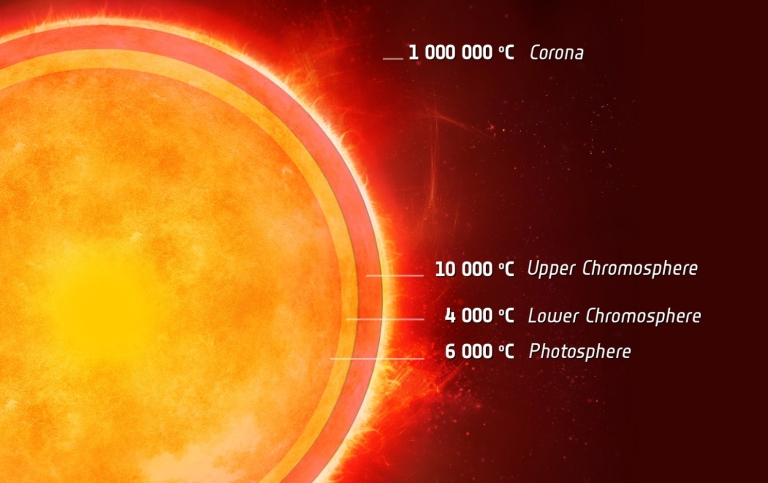
\includegraphics[width=9cm]{figures/stellatm.jpg}
\caption{Scheme of the stellar atmosphere. Credits: ESA}
\end{figure}
}
%
\frame{
\frametitle{Interior vs atmosphere relationships}
\begin{itemize}
%\item The stellar light gives us direct information about the stellar surface (the photosphere).
\item Stellar structure determines the structure of the atmosphere, and $T_{\rm eff}$.
\item Stellar atmosphere oscillates because of the processes in stellar interior. 
\item At the surface, we measure the magnetic fields generated in the interior. 
\item Neutrinos produced in the core leave the star directly. 
\item \textbf{The structure of the whole star leaves an observable imprint on its surface.}
\end{itemize}
}
%
\frame{
\frametitle{Understanding the stars}
\begin{minipage}{0.495\linewidth}
\begin{itemize}
\item \textbf{The structure of the whole star leaves an observable imprint on its surface.}
\item We measure these observable imprints. 
\item We can observe \emph{a lot} of stars - so we can have accurate statistics. 
\item \textbf{We devise theoretical models that try to describe the stellar structure and the evolution and compare the outputs of these models both to the measurable properties of individual stars and to the statistical distributions.}
\end{itemize}
\end{minipage}
\hfill
\begin{minipage}{0.495\linewidth}
\begin{figure}
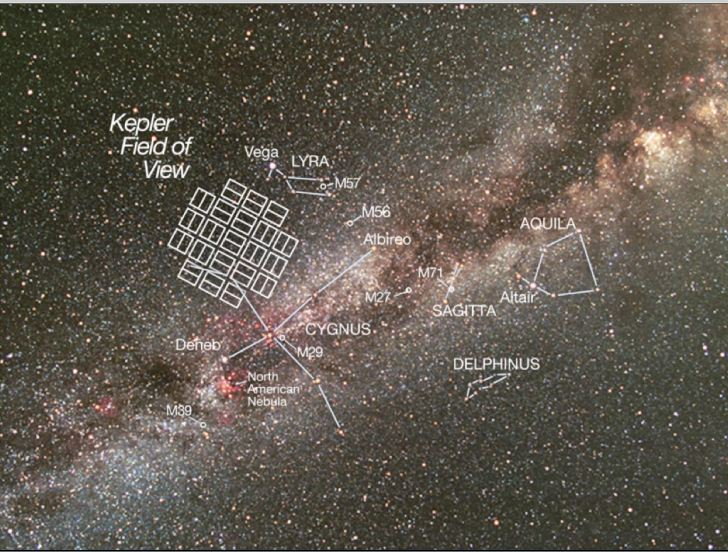
\includegraphics[width=6cm]{figures/kepler_fov.jpg}
\caption{Kepler mission field of view. Credits: NASA}
\end{figure}
\end{minipage}
}
%
\section{Stellar colors}
%
\frame{
\frametitle{Luminosity vs the color}
\begin{itemize}
\item Effective temperature describes the total luminosity of the star.
\item We used a blackbody to approximate solar \emph{surface} - \textbf{not the whole star!}.
\item Now, different temperatures imply different colors (i.e. different spectral distributions).
\begin{figure}
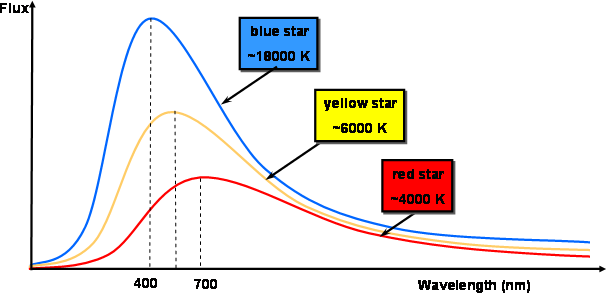
\includegraphics[width=7.5cm]{figures/bb_curves.png}
\caption{Planck curves for blackbodies of different temperatures. Credits: University of Swinburne}
\end{figure}
\end{itemize}
}
%
\frame{
\frametitle{Stars are not black bodies!}
\begin{itemize}
\item Star needs to transport energy outwards. For that a gradient of temperature is needed - not a blackbody. 
\item \q{Harder question is: can stellar photosphere be a blackbody?}
\item We leave that for a different discussion, but in short: 
\item It cannot, although we can roughly approximate it as: 
\item Blackbody radiation + additional absorption/emission in the stellar \emph{atmosphere}.
\end{itemize}
}
%
\frame{
\frametitle{Solar spectrum is NOT a blackbody spectrum}
\begin{figure}
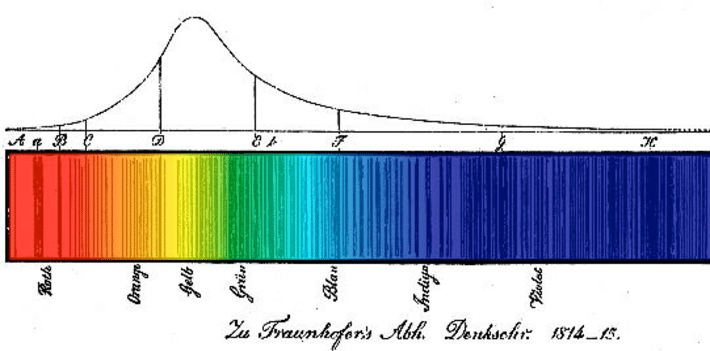
\includegraphics[width=10cm]{figures/fraunhofer_spectrum.png}
\caption*{Credits: Fraunhofer (1814)}
\end{figure}
\begin{itemize}
\item Wollastone (1802) and Fraunhofer (1814) discovered dark lanes in the solar spectrum,
\item These lines represent loss of light at specific wavelengths - solar atmosphere is much more opaque at these wavelengths. \q{Why?}
\end{itemize}
}
%
%
\frame{
\frametitle{Solar spectrum is NOT a blackbody spectrum}
\begin{figure}
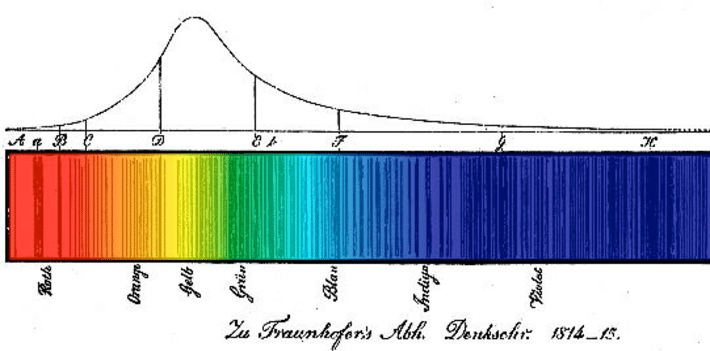
\includegraphics[width=6cm]{figures/fraunhofer_spectrum.png}
\caption*{Credits: Fraunhofer (1814)}
\end{figure}
\begin{itemize}
\item These lines represent loss of light at specific wavelengths - solar atmosphere is much more opaque at these wavelengths. \q{Why?}
\item Kirchoff and Bunsen (1860's) related them to chemical elements. 
\item Birth of quantum mechanics: Bohr's model can explain hydrogen lines. \textbf{Energy jumps between discrete energy levels}.
\item Discovery of Helium by Janssen (1868) in the solar spectrum.
\end{itemize}
}
%
%
\frame{
\frametitle{Planck Law}
\begin{itemize}
\item Kirchoff (again) reckognized the importance of an universal law that connects emission and absorption properties of a medium in an equilibrium state. - \emph{"... It is of utmost importance to derive this law theoretically"}. 
\item We had some pieces: Stefan-Boltzmann law that we just talked about...
\item ... the Wien's law: Emission of bodies of different temperature peaks at different wavelengths (colors).
\item People also experimentally captured the dependence $B(T)$, where $B$ is the emitted flux density.
\item \emph{Interesting:} Both Boltzmann and Wien (as well as Rayleigh and later Jeans) derived the corresponding laws theoretically. \q{Do you know how?}
\item Recommendation: ``Theoretical Concepts in Physics'' (Malcom Longair, 2020, Cambridge)
\end{itemize}
}
%
\frame{
\frametitle{Planck Law}
\begin{minipage}{0.5\linewidth}
\begin{itemize}
\item Finally, Planck derived this law theoretically. 
\item After that, multiple other approaces to derivation were made (for example one by Bose and Einstein).
\begin{equation}
B(\lambda, T) = \frac{2hc^2}{\lambda^5} \frac{1}{e^{hc/\lambda k T} - 1}
\end{equation}
\item This equation describes the \emph{intensity} of the light in a state where photons are in equilibrium. 
\end{itemize}
\end{minipage}
\hfill
\begin{minipage}{0.49\linewidth}
\begin{figure}
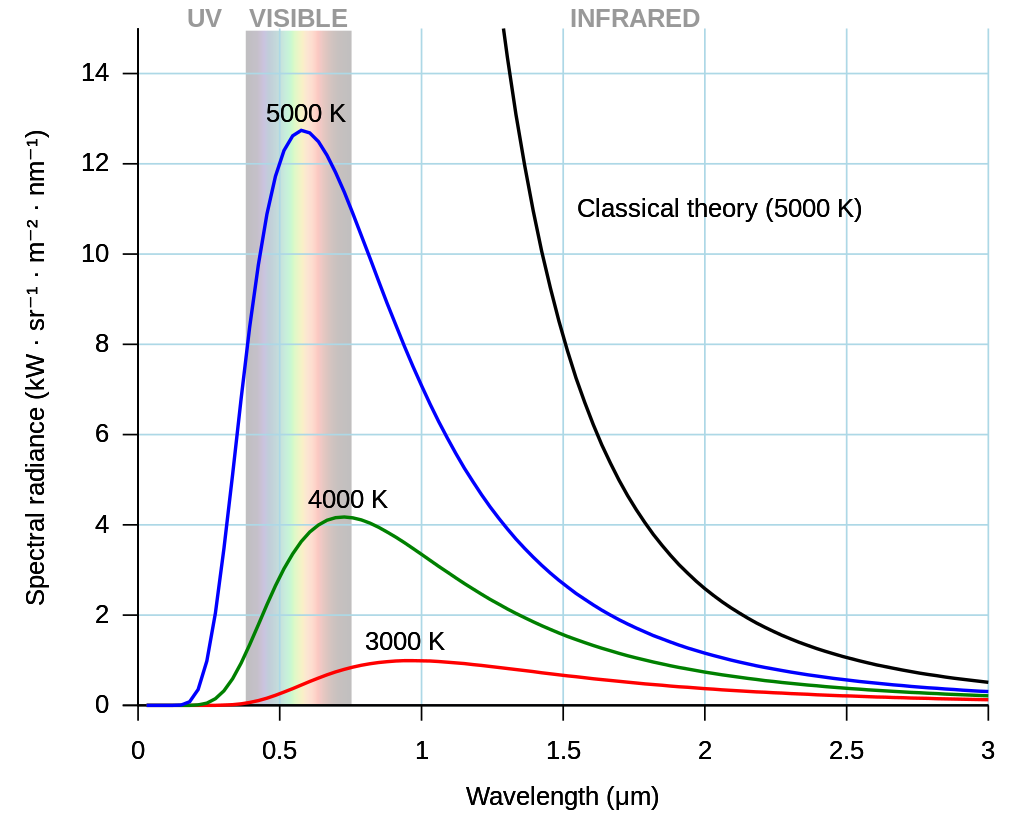
\includegraphics[width=8cm]{figures/b_b2.png}
\caption*{Planck curves for few different temperatures. Credits: Wikipedia}
\end{figure}
\end{minipage}
}
%
%
\frame{
\frametitle{Solar spectrum is NOT a blackbody spectrum}
\begin{figure}
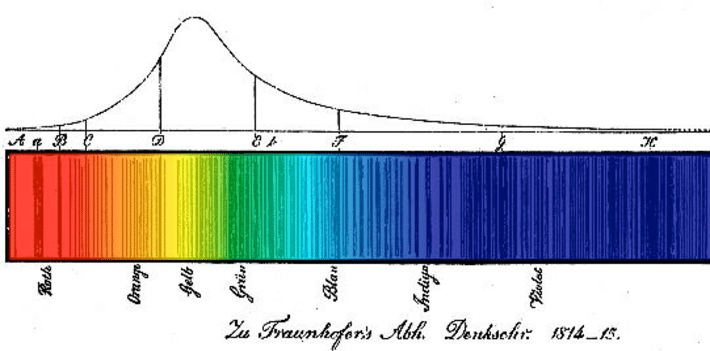
\includegraphics[width=6cm]{figures/fraunhofer_spectrum.png}
\caption*{Credits: Fraunhofer (1814)}
\end{figure}
\begin{itemize}
\item These lines represent loss of light at specific wavelengths - solar atmosphere is much more opaque at these wavelengths. \q{Why?}
\item Kirchoff and Bunsen (1860's) related them to chemical elements. 
\item Birth of quantum mechanics: Bohr's model can explain hydrogen lines. \textbf{Energy jumps between discrete energy levels}.
\item Discovery of Helium by Janssen (1868) in the solar spectrum.
\end{itemize}
}
%
\frame{
\frametitle{Today we can do better than 200 years ago ...}
\begin{figure}
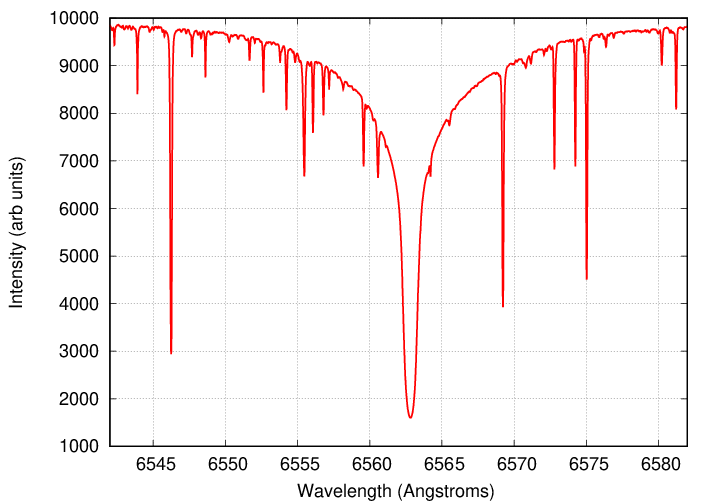
\includegraphics[width=8cm]{figures/sun_halpha_a.png}
\caption*{H$\alpha$ spectral line in solar spectrum: notice all the weak spectral lines around!}
\end{figure}
}
%
\frame{
\frametitle{And we can do the same for other stars.}
\begin{figure}
\begin{tabular}{cc}
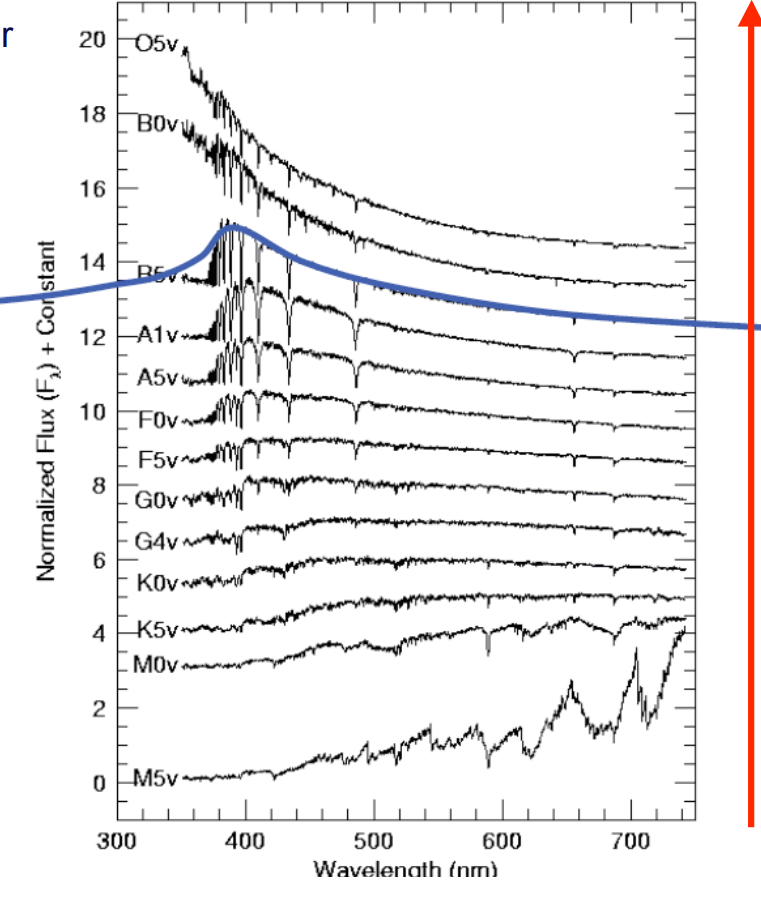
\includegraphics[width=9cm]{figures/spectra_stars.png}
\end{tabular}
\caption*{Credits: Adam Burrows, Princeton}
\end{figure}
}
%
%
\frame{
\frametitle{And we can do the same for other stars.}
\begin{minipage}{0.45\linewidth}
\q{What is the fundamental parameter that determines the shape of the spectrum and the absence/presence of spectral lines?}
\end{minipage}
\hfill
\begin{minipage}{0.54\linewidth}
\begin{figure}
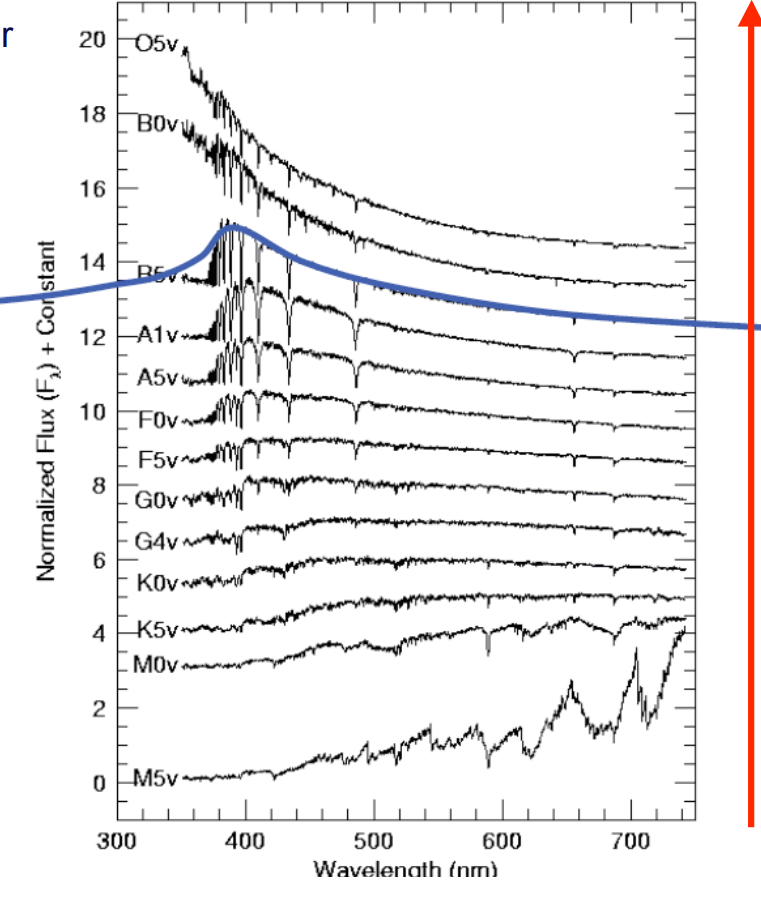
\includegraphics[width=6cm]{figures/spectra_stars.png}
\caption*{Credits: Adam Burrows, Princeton}
\end{figure}
\end{minipage}
}
%
%
\frame{
\frametitle{And we can do the same for other stars.}
\begin{minipage}{0.45\linewidth}
\q{What is the fundamental parameter that determines the shape of the spectrum and the absence/presence of spectral lines?}
\vspace{1cm}\\
It is the temperature! It determines the ionization and excitation of the particles and thus their absorption/emission properties.
\end{minipage}
\hfill
\begin{minipage}{0.54\linewidth}
\begin{figure}
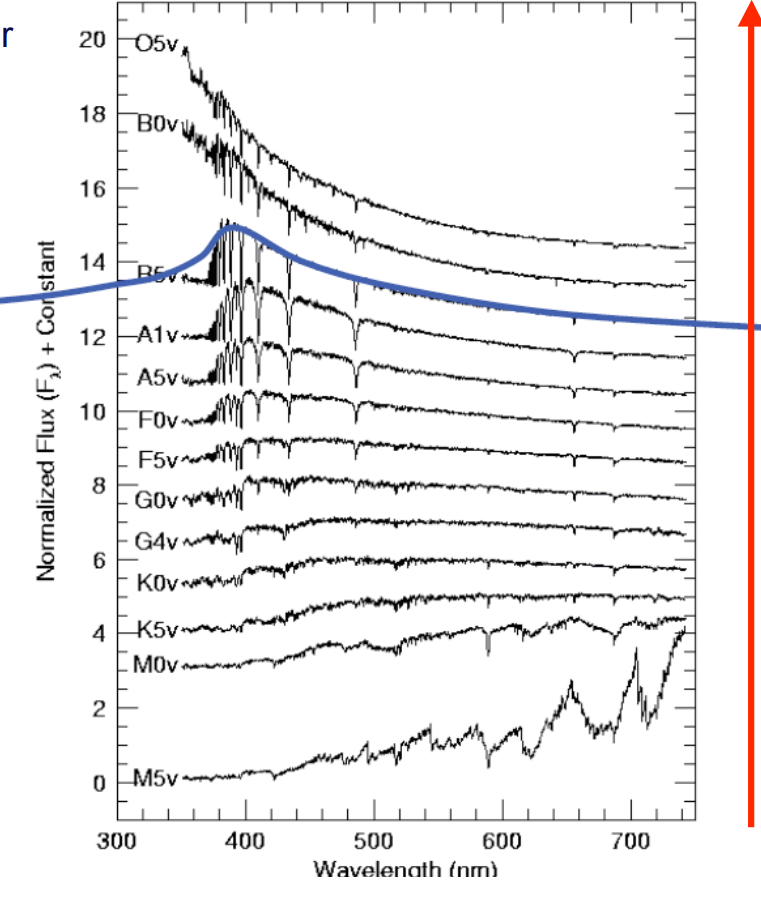
\includegraphics[width=6cm]{figures/spectra_stars.png}
\caption*{Credits: Adam Burrows, Princeton}
\end{figure}
\end{minipage}
}
%

\frame{
\frametitle{The Harvard Spectral Classification}
\begin{minipage}{0.48\linewidth}
\begin{tabular}{cc}
Class & \red{T$_{\rm eff}$} [K] \\
\hline
O & $\ge$ 30000 \\
B & 10000-30000 \\
A & 7500-10000 \\
F & 6000-7500 \\
G & 5000-6000 \\
K & 3000-5000 \\
M & 2000-3000 
\end{tabular}
\end{minipage}
\hfill
 \begin{minipage}{0.48\linewidth}
\begin{figure}
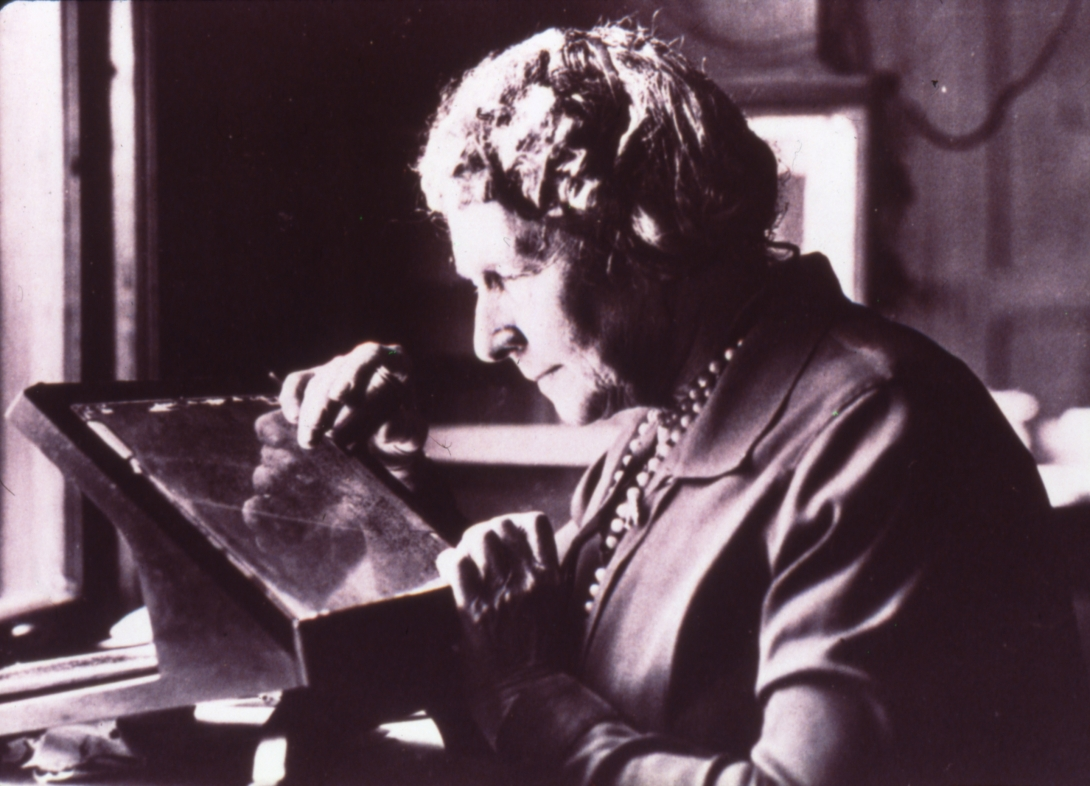
\includegraphics[width=6cm]{figures/ajc.jpg}
\caption*{Annie Jump Cannon. Credits: Library of Congress, US}
\end{figure}
\end{minipage}
}
%
\frame{
\frametitle{HR diagram: basics}
\begin{minipage}{0.48\linewidth}
\begin{itemize}
\item There are three groups of stars.
\item For one (main sequence) the color and brightness are somewhat correlated.
\item Other is very hot but faint - white dwarves
\item The last is cool but bright - (red) giants (there are also other giants).
\item It will turn out these are \emph{phases} in stellar evolution.
\end{itemize}
\end{minipage}
\hfill
\begin{minipage}{0.48\linewidth}
\begin{figure}
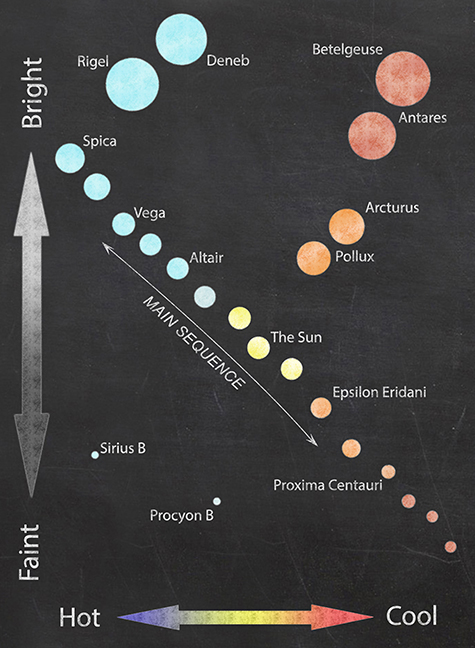
\includegraphics[width=5.2cm]{figures/hr_simple.jpg}
\caption*{Credits: the Open University}
\end{figure}
\end{minipage}
}
%
%
\frame{
\frametitle{HR diagram: basics}
\begin{minipage}{0.48\linewidth}
\begin{itemize}
\item It will turn out these are \emph{phases} in stellar evolution.
\item We \textbf{can't} observe stars as they evolve and age.
\item But we can observe a lot of stars and try to infer things. 
\item It is like aliens observed us very briefly: they would need some time that small, weak humans are a first stage in a lifetime of a human being.
\end{itemize}
\end{minipage}
\hfill
\begin{minipage}{0.48\linewidth}
\begin{figure}
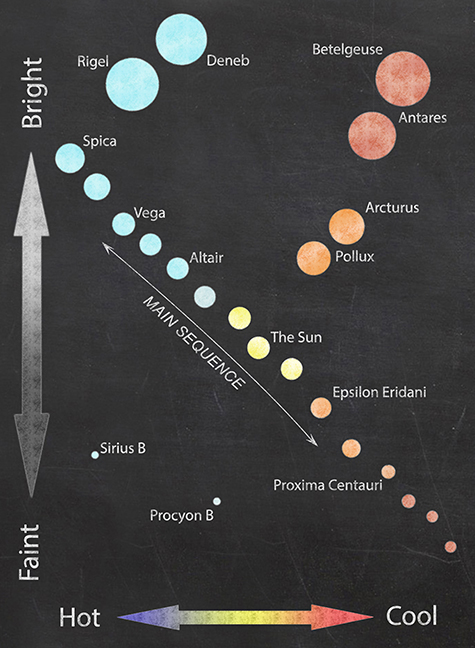
\includegraphics[width=5.2cm]{figures/hr_simple.jpg}
\caption*{Credits: the Open University}
\end{figure}
\end{minipage}
}
%
%
\frame{
\frametitle{HR diagram: questions}
\begin{minipage}{0.48\linewidth}
\begin{itemize}
\item Why are the color and the brightness of the stars on the main sequence correlated?
\item In which order these evolutionary stages take place?
\item What determines when and how the star changes between these stages?
\item What are the fundamental differences between these phases?
\end{itemize}
\end{minipage}
\hfill
\begin{minipage}{0.48\linewidth}
\begin{figure}
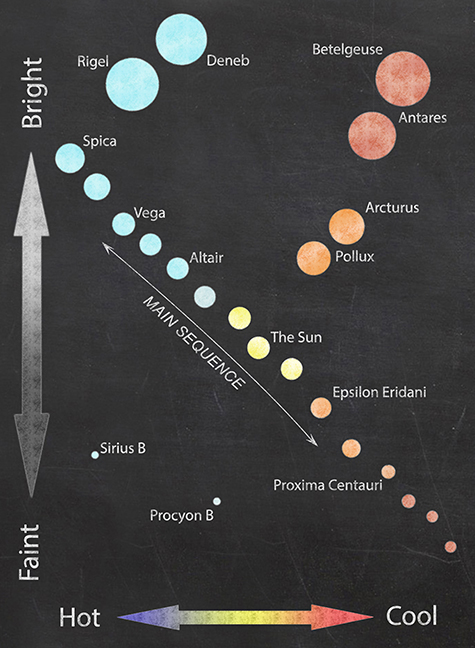
\includegraphics[width=5.2cm]{figures/hr_simple.jpg}
\caption*{Credits: the Open University}
\end{figure}
\end{minipage}
}
%
\frame{
\frametitle{How can we infer other stellar parameters?}
\begin{itemize}
	\item We saw that we can estimate luminosity from the apparent brightness (irradiance) and distance. 
	\item And that we can infer the effective temperature from the color.
	\item Combined, these two give us the radius (this will be your homework).
	\item What about the mass? Physical composition? Magnetic field? Rotation rate?
\end{itemize}
}
%
\frame{
\frametitle{Stellar masses}
\begin{minipage}{0.44\linewidth}
\begin{itemize}
\item Are extremely important, yet extremely hard to infer.
\item The only accurate opportunity to infer the mass is to observe the star in a dynamical interaction.
\item For example in a binary system. 
\item Very important, a big fraction of the stars are in binary (or multiple systems).
\item The stars can also interact with each other. 
\end{itemize}
\end{minipage}
\hfill
\begin{minipage}{0.55\linewidth}
\begin{figure}
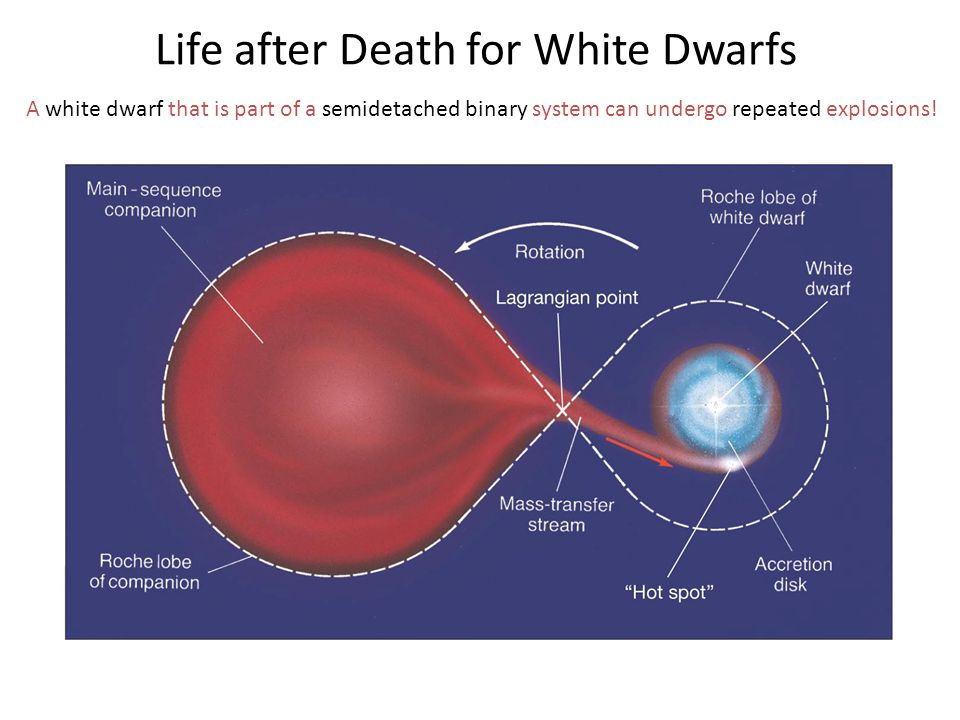
\includegraphics[width=7.6cm]{figures/roche_lobe.jpg}
\end{figure}
\end{minipage}
}
%
\frame{
\frametitle{Element abundances in the Universe }
\begin{minipage}{0.4\linewidth}
\begin{itemize}
\item Most of these elements were generate in stars. 
\item But they also have implications for generation and evolution of other stars? 
\item \q{Let's have a relaxed discussion on importance of heavier elements.}
\end{itemize}
\end{minipage}
\hfill
\begin{minipage}{0.59\linewidth}
\begin{figure}
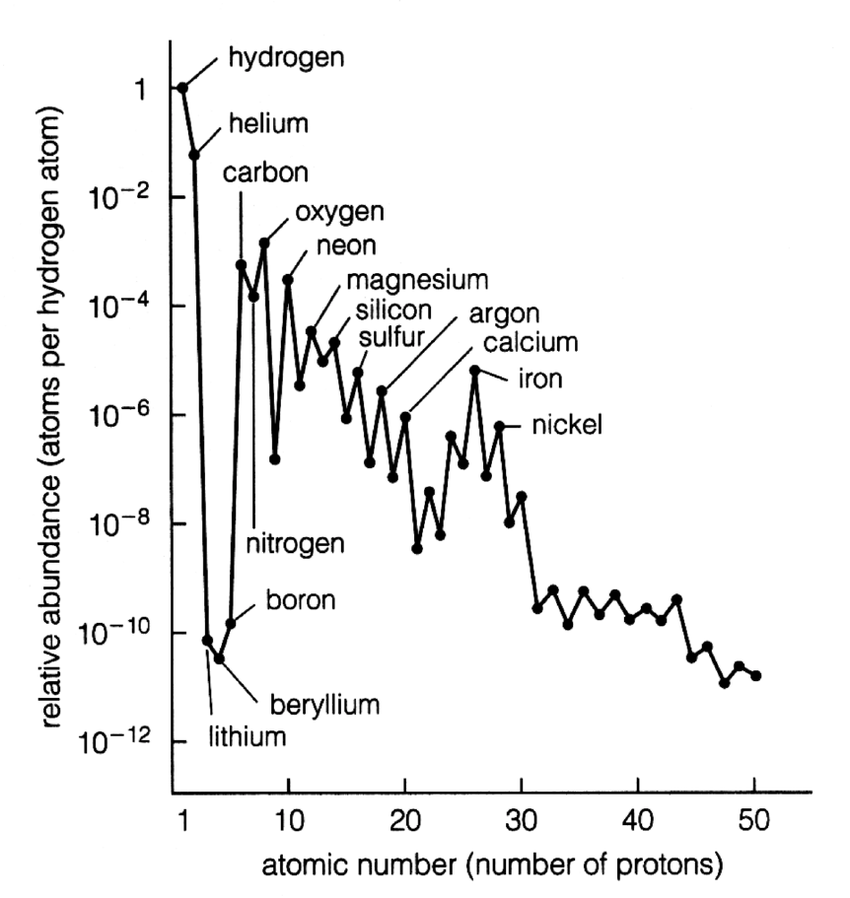
\includegraphics[width=7cm]{figures/The-relative-abundances-of-elements-in-the-universe-after-Goldschmidt-1938.png}
\caption*{Credits: Goldschmidt 1938}
\end{figure}
\end{minipage}
}
%
\frame{
\frametitle{These abundances are inferred from the spectra}
\begin{minipage}{0.495\linewidth}
\begin{itemize}
\item Determination of the Silicon Abundance by fitting the solar spectra
\item \sepia{Dots}: observations; \sepia{dashed/solid}: low/high Silicon abundance.
\end{itemize}
\end{minipage}
\hfill
\begin{minipage}{0.495\linewidth}
\begin{figure}
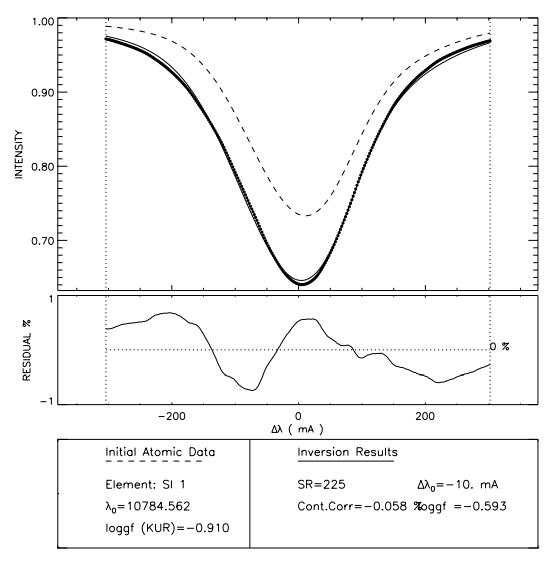
\includegraphics[width=6cm]{figures/abundance_si.png}
\caption*{Credits: Borrero et al. 2003}
\end{figure}
\end{minipage}
}
%
%
\section{Stellar modeling}
\frame{
	\frametitle{What is the goal of stellar structure and evolution modeling?}
	\begin{minipage}{0.495\linewidth}
	\begin{itemize}
		\item To explain why are luminosity and temperature correlated.
		\item To understand what determines these two parameters. 
		\item To predict/reconstruct the evolutionary paths of stars on HR diagram.
		\item Little bit further down the road: to understand changes in stars on various scales (pulsations, oscillations), stellar magnetic field generation, stellar activity and the interaction between the stars and their environment. 
	\end{itemize}
	\end{minipage}
	\hfill
	\begin{minipage}{0.495\linewidth}
	\begin{figure}
	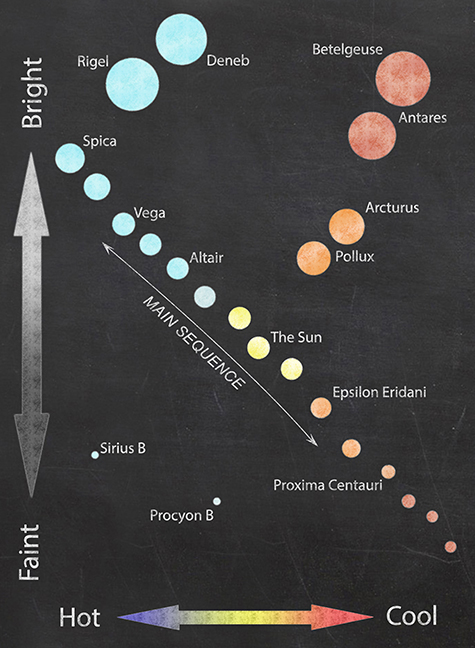
\includegraphics[width=5.2cm]{figures/hr_simple.jpg}
	\caption*{Credits: the Open University}
	\end{figure}
	\end{minipage}
}
%

\frame{
	\frametitle{Basic assumptions - what we are working with}
	\begin{minipage}{0.495\linewidth}
	\begin{itemize}
		\item Star exists and evolves in isolation.
		\item The star is non-rotating and spherically symmetric. 
		\item The star is uniform in it's initial composition. 
		\item We ignore the effect of magnetic fields. 
	\end{itemize}
	\end{minipage}
	\hfill
	\begin{minipage}{0.495\linewidth}
	\begin{figure}
	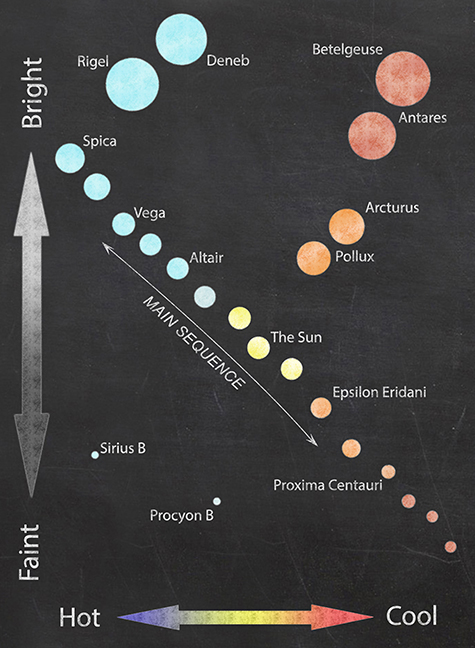
\includegraphics[width=5.2cm]{figures/hr_simple.jpg}
	\caption*{Credits: the Open University}
	\end{figure}
	\end{minipage}
}
%
\frame{
	\frametitle{How to play the game}
	\begin{minipage}{0.495\linewidth}
	\begin{itemize}
		\item We describe our star as a radial distribution of temperature, pressure and density. 
		\item We also describe it through it's chemical composition.
		\item These parameters will be connected with some differential equations. 
		\item Solving them should give us observable parameters ($T_eff$, $L$) for given boundary conditions. 
		\item When we let the system evolve, we should be able to reproduce the evolution of stars on the HR diagram.
	\end{itemize}
	\end{minipage}
	\hfill
	\begin{minipage}{0.495\linewidth}
	\begin{figure}
	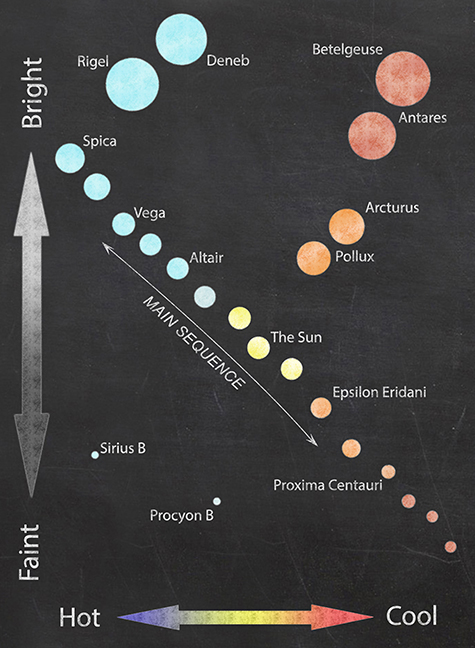
\includegraphics[width=5.2cm]{figures/hr_simple.jpg}
	\caption*{Credits: the Open University}
	\end{figure}
	\end{minipage}
}

\frame{
	\frametitle{The coordinate system}
	\begin{minipage}{0.6\linewidth}
	\begin{itemize}
		\item Problem is 1D - it is natural to describe variation of physical quantities with radius: $T(r),\,\rho(r)\,p(r)$. I.e. we consider \emph{layers} with thickness $dr$
		\item Alternatively, we can focus on \emph{elements} that enclose some very small mass $dm$. 
		\item This is Eulerian vs Lagrangian formulation. We will use them both.
		\item The first one is more intuitive, the second more useful when the star dimensions change.
		\item They are connected as (conservation of mass):
		\begin{equation}
		dm = \rho(r) 4\pi r^2 dr
		\end{equation}
	\end{itemize}
	\end{minipage}
	\hfill
	\begin{minipage}{0.4\linewidth}
	%\begin{figure}
	%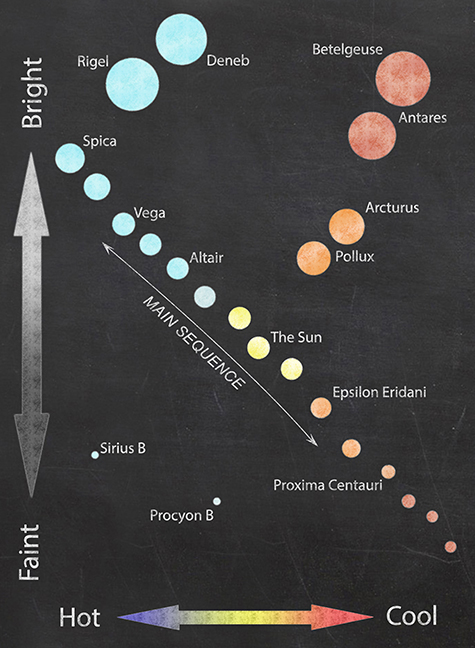
\includegraphics[width=5.2cm]{figures/hr_simple.jpg}
	%\caption*{Credits: the Open University}
	%\end{figure}
	\end{minipage}
}

\frame{
	\frametitle{The energy equation}
	\begin{minipage}{0.6\linewidth}
	\begin{itemize}
		\item Energy is flowing through a parcel. It can also be generated in the parcel (if we have a source).
		\begin{equation}
		\delta (u dm) = dm \delta u = \delta Q + \delta W
		\end{equation}
		\item where $Q$ is amount of heat, and $W$ is work. Then
		\begin{equation}
		\delta W = -p \delta dV = -p \frac{1}{\rho} \delta dm.
		\end{equation}
		\begin{equation}
		\delta Q = q dm \delta t + F(m) \delta t - F(m+ dm) \delta t
		\end{equation}
		\begin{equation}
		\delta Q = (q-\frac{\partial F}{\partial m} dm \delta t)
		\end{equation}
	\end{itemize}
	\end{minipage}
	\hfill
	\begin{minipage}{0.4\linewidth}
	%\begin{figure}
	%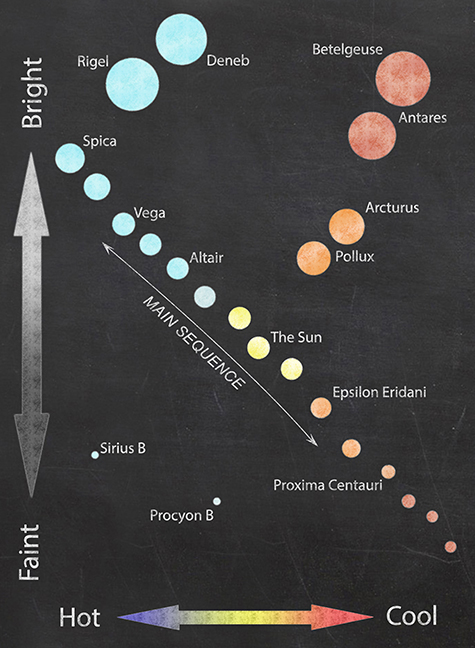
\includegraphics[width=5.2cm]{figures/hr_simple.jpg}
	%\caption*{Credits: the Open University}
	%\end{figure}
	\end{minipage}
}

\frame{
	\frametitle{The energy equation}
	\begin{minipage}{0.6\linewidth}
	\begin{itemize}
		\item Now, taking the limit of a small $\delta t$, and putting these two together we have:
		\begin{equation}
		\dot{u} + p \dot{(\frac{1}{\rho})} = q - \frac{dF}{dm}
		\end{equation}
		\item Which, for the moment, we are going to consider to be static:
		\begin{equation}
		q = \frac{dF}{dm}
		\end{equation}
		\item In the absence of sources $F$ is constant. $F$ at surface needs to be $L$. This power is supplied by the nuclear processes (i.e. nuclear luminosity):
		\begin{equation}
		L_{\rm nuc} = \int_0^{M} q dm.
		\end{equation}	
	\end{itemize}
	\end{minipage}
	\hfill
	\begin{minipage}{0.4\linewidth}
	%\begin{figure}
	%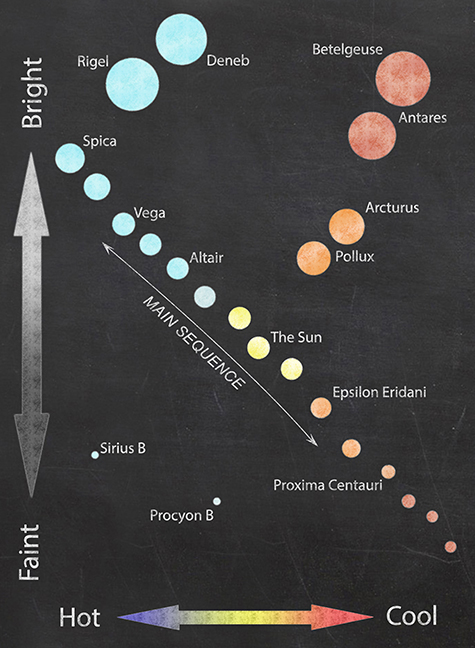
\includegraphics[width=5.2cm]{figures/hr_simple.jpg}
	%\caption*{Credits: the Open University}
	%\end{figure}
	\end{minipage}
}

\frame{
	\frametitle{The equation of motion}
	\begin{minipage}{0.6\linewidth}
	\begin{itemize}
		\item Analyzing the forces acting on the element: 
		\begin{equation}
		\ddot{r} = -G\frac{m}{r^2} - \frac{\partial p}{\partial r} \frac{1}{\rho}.
		\end{equation}
		\item Or, if we work in $dm$:
		\begin{equation}
		\ddot{r} = -G\frac{m}{r^2} - 4\pi r^2\frac{\partial p}{\partial m} .
		\end{equation}
	\end{itemize}
	\end{minipage}
	\hfill
	\begin{minipage}{0.4\linewidth}
	%\begin{figure}
	%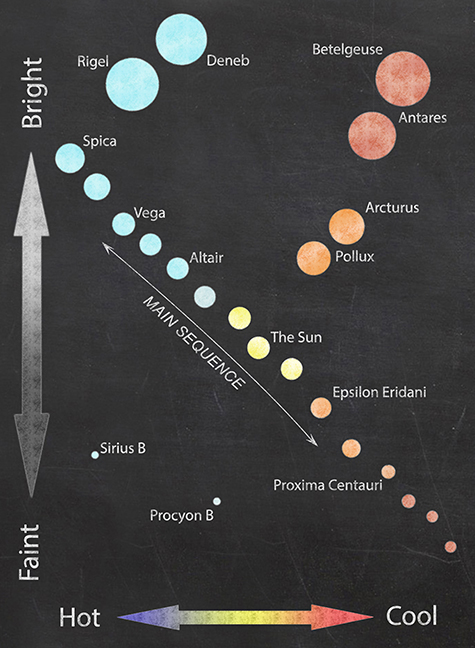
\includegraphics[width=5.2cm]{figures/hr_simple.jpg}
	%\caption*{Credits: the Open University}
	%\end{figure}
	\end{minipage}
}

\frame{
	\frametitle{Hydrostatic equilibrium}
	\begin{minipage}{0.6\linewidth}
	\begin{itemize}
		\item If the star is static, there are no accelerations:
		\begin{equation}
		\frac{dp}{dr} = -\rho \frac{Gm}{r^2},
		\end{equation}
		\item or in $dm$:
		\begin{equation}
		\frac{dp}{dm} = -G\frac{m}{4\pi r^2}
		\end{equation}
		\item Estimate the pressure at the center:
		\begin{equation}
		p_c = \int_0^M \frac{G m dm}{4\pi r^2} > \int_0^M \frac{G m dm}{4\pi r^2} 
		\end{equation}
		
	\end{itemize}
	\end{minipage}
	\hfill
	\begin{minipage}{0.4\linewidth}
	%\begin{figure}
	%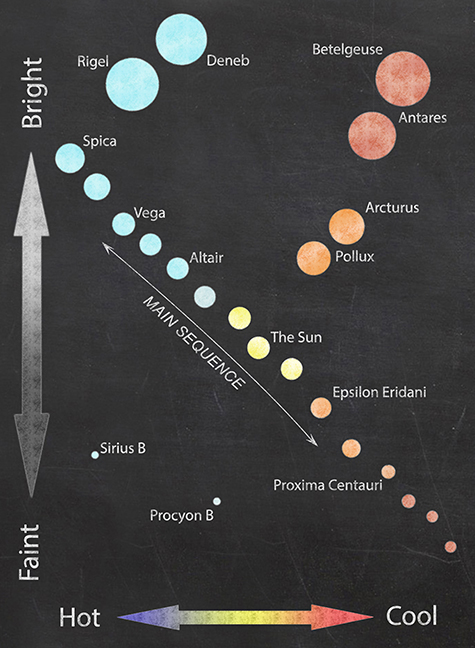
\includegraphics[width=5.2cm]{figures/hr_simple.jpg}
	%\caption*{Credits: the Open University}
	%\end{figure}
	\end{minipage}
}

\frame{
	\frametitle{Virial theorem}
	\begin{minipage}{0.6\linewidth}
	
	\end{minipage}
	\hfill
	\begin{minipage}{0.4\linewidth}
	%\begin{figure}
	%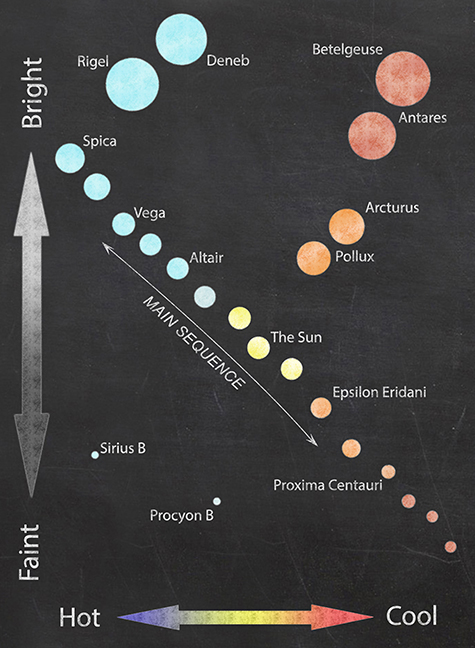
\includegraphics[width=5.2cm]{figures/hr_simple.jpg}
	%\caption*{Credits: the Open University}
	%\end{figure}
	\end{minipage}
}

\frame{
	\frametitle{Total energy of the star}
	\begin{minipage}{0.6\linewidth}
	
	\end{minipage}
	\hfill
	\begin{minipage}{0.4\linewidth}
	%\begin{figure}
	%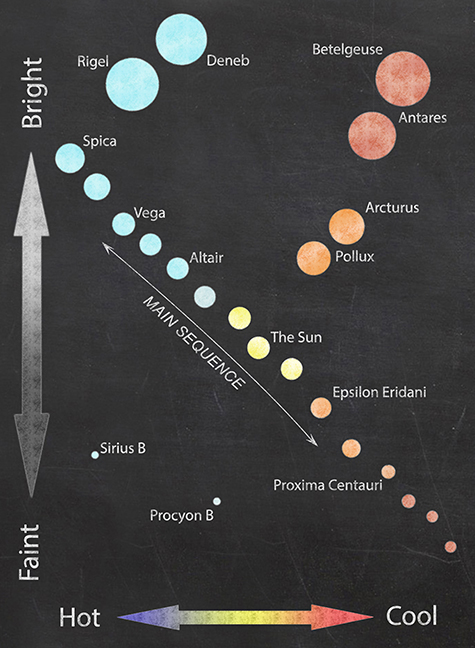
\includegraphics[width=5.2cm]{figures/hr_simple.jpg}
	%\caption*{Credits: the Open University}
	%\end{figure}
	\end{minipage}
}

\frame{
	\frametitle{Contracting = losing energy = heating}
	\begin{minipage}{0.6\linewidth}
	
	\end{minipage}
	\hfill
	\begin{minipage}{0.4\linewidth}
	%\begin{figure}
	%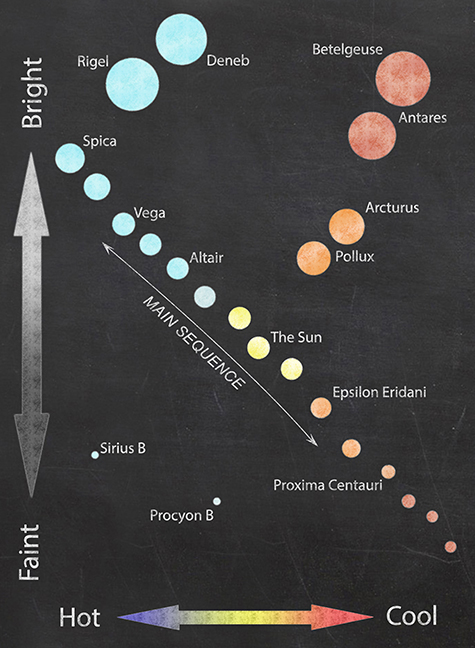
\includegraphics[width=5.2cm]{figures/hr_simple.jpg}
	%\caption*{Credits: the Open University}
	%\end{figure}
	\end{minipage}
}



\frame{
\frametitle{Question to think about}
\begin{itemize}
	\item We said that the effective temperature of the Sun is $5777$\,K.
	\item We also said that this temperature is not constant, but must be increasing inward, in order to drive energy flux outward.
	\item \q{What is the temperature in the core?}
	\item \q{What is the source of energy?}
\end{itemize}
}
%
\frame{
\frametitle{Answer}
\begin{itemize}
	\item The temperature at the core is $\approx 1.5\times 10^7$\,K. And the source of energy is nuclear fusion of $H$ in $He$. 
	\item How do we know? It took us some time. 
	\item First one to even think about this was Eddington. (Maybe check \href{https://arxiv.org/pdf/2111.02096.pdf}{this} paper by H. Kragh).
	\item The previous idea was graviational contraction. 
	\item The temporal scale for such a process is the \textbf{Kelvin-Helmholtz timescale}.
\end{itemize}
}
%
\frame{
\frametitle{Kelvin-Helmholtz timescale}
\begin{itemize}
	\item Let's do an order of magnitude estimation:
	\begin{equation}
	t_{\rm KH} = \frac{GM^2}{RL}
	\end{equation}
	\item For the Sun this amounts to 30 million years. 
	\item We knew back then already that Earth is billions of years old. 
	\item It had to be something else!
\end{itemize}
}
%
\frame{
\frametitle{Nuclear timescale}
\begin{itemize}
	\item Let's do an order of magnitude estimation:
	\begin{equation}
	t_{\rm KH} = \frac{GM^2}{RL}
	\end{equation}
	\item For the Sun this amounts to 30 million years. 
	\item We knew back then already that Earth is billions of years old. 
	\item It had to be something else!
\end{itemize}
}
%
\frame{
\frametitle{Dynamical timescale}
\begin{itemize}
	\item Let's do an order of magnitude estimation:
	\begin{equation}
	t_{\rm KH} = \frac{GM^2}{RL}
	\end{equation}
	\item For the Sun this amounts to 30 million years. 
	\item We knew back then already that Earth is billions of years old. 
	\item It had to be something else!
\end{itemize}
}
\end{document}



